\section{Complex Numbers}
A complex number is a number of the form
\begin{equation}
z = a + i b
\label{zrect}
\end{equation}
where the imaginary unit is defined as
\footnote{In electrical engineering,
a lower case $i$ represents a time-dependent current, so it is
their convention to use the symbol $j$ in place of $i$.}
\begin{equation}
i = \sqrt{-1}
\label{idef}
\end{equation}
and $a$ is the real part of $z$, written $a = Re(z)$, and $b$ is the 
imaginary part of $z$, written $b = Im(z)$.     $a$ and
$b$ are real numbers. 

Complex numbers have real and imaginary parts.
However, if a number has no real part, then it is called
`pure imaginary'.


It may be easily verified 
from Eq. (\ref{idef}) that $i^2 = -1$, and that
\begin{equation}
\frac{1}{i} = -i
\end{equation}

\section{The Complex Plane}
A complex number can be visualized in a
two-dimensional number line, known as an 
Argand diagram, or the complex plane
as shown in Fig. \ref{argand}.
\begin{figure}
\begin{center}
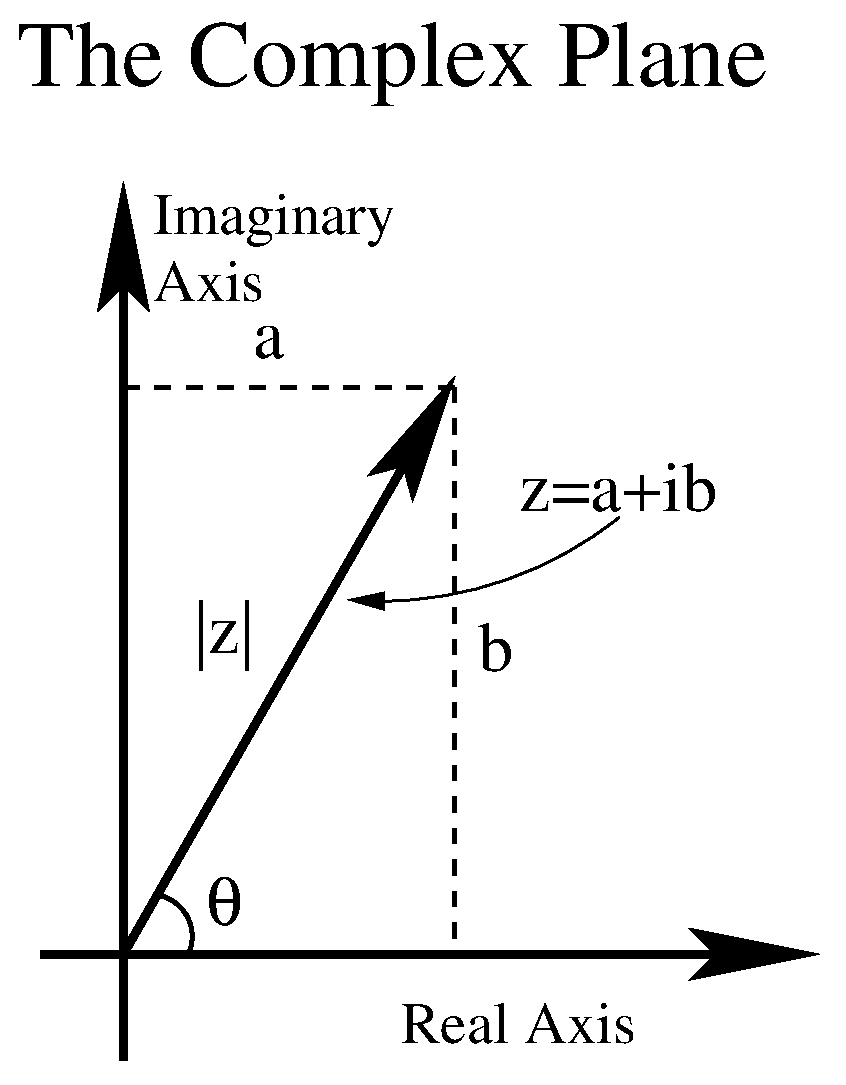
\includegraphics[width=5cm,height=5cm]{images/argand.eps}
\caption[The Complex Plane]{A complex number is easily visualized as
a "phasor" in the complex plane.}
\label{argand}
\end{center}
\end{figure}
The complex plane replaces the number line as a visualization
tool for real numbers.  However, rather than plot points
in the complex plane, it is conventional to represent
a complex number as a vector in the complex plane.  Instead
of calling them complexified vectors, they are referred to
as ``phasors.''  Note 
that because the visualization
is 2-dimensional, a polar form for complex numbers is suggested.
This is discussed below.%  

As an addition side note about the 
complex plane, complex analysis can be used to study
improper real integrals that couldn't otherwise be
solved.  Basically, for an integral that extends from
$-\infty$ to $\infty$, instead of integrating over
the real number line, one may perform a closed path line
integral that includes the real number line and a semicircle
of radius $R$, which is allowed to approach $\infty$.
The residue theorem relates the closed loop integral
to a real value.  However, it can be shown that the
integral over the infinite semicircle approaches zero,
and our integral of interest is obtained.

\section{Complex Magnitude}
From Fig. \ref{argand}, it can be easily seen (using the Pythagorean theorem) 
that the magnitude, or length, of the vector representing
a complex number is
\begin{equation}
|z| = \sqrt{a^2 + b^2}
\end{equation}
Thus, the complex magnitude is the 
square root of the sum of the squares of the real 
and imaginary parts of the complex number.
This definition generalizes the absolute value
function of a real number.

\section{Complex Conjugate}
The complex conjugate of a complex number $z$, is denoted
$\bar{z}$, and is defined
\[
\bar{z} = a - i b
\label{zconjrect}
\]
We may think of the conjugation process as
``replacing $i$ with $-i$.''

Where would the vector $\bar{z}$ fit on the complex plane in Fig \ref{argand}?

\begin{example}[Complex Conjugate]
Prove that $\bar{z}z = |z|^2$.
\end{example}
\begin{proof}
\begin{eqnarray*}
\bar{z}z &=& (a - ib)(a+ib) \\
&=& a^2 + b^2 \\
&=& (a^2 + b^2)^{1/2} (a^2 + b^2)^{1/2} \\
&=& \samepage |z|^2
\end{eqnarray*}
\end{proof}
Note that $\bar{z}z$ is real and positive.  A quotient of complex numbers can 
be written separated 
into real and imaginary parts using the above conjugate relation
as shown in the next example.

\begin{example}
\textbf{Complex Fractions}\\
Separate the complex number $z = \frac {3-i4}{5+i12}$
into real and imaginary parts.
\end{example}
\begin{proof}
The solution involves the well known rationalizing 
the denominator technique of multiplying the top and bottom of the quotient 
by the conjugate of the denominator.

\begin{eqnarray*}
z &=& \frac {3-i4}{5+i12} \\
  &=& \frac {3-i4}{5+i12} \frac {5-i12}{5-i12}  \\
  &=& \frac {(15-48)+i(-20-36)}{13} \\
  &=& - \frac {33+i56}{13} 
\end{eqnarray*}
\end{proof}
It may be noted that $|\bar{z}| = |z|$.  Also, the conjugate of a product 
is a product of conjugates so that $\overline{(uv)} = \bar{u} \bar{v}$.  Similarly, 
the conjugate of a sum is the sum of conjugates so that 
$\overline{(u + v)} = \bar{u} + \bar{v}$.
Finally, the conjugate of a conjugate is the function itself, i.e.
$\overline{(\overline{z})} = z$.  Put another way, complex conjugation ``toggles.''

\begin{example}
Consider the function $f(z) = 3z^2 +(2+i7)z + i6$ where $z$ is 
a complex variable. \\
\indent
a)      What is the conjugate of  the function, $f^*(z)$? \\
\indent
b)      What is $f(\bar{z})$? \\
\indent
c)      What is $f^*(\bar{z})$? \\
\end{example}

\begin{proof}
Following the simple steps:
\begin{eqnarray*}
a)  f^*(z) &=& [3z^2 + (2+i7)z + i6]^* \\
           &=& (3z^2)^* + [(2+i7)z]^* + (i6)^* \\
           &=& 3z^{*2} +[(2+i7)^*\bar{z}] +i^*6^* \\
           &=& 3z^{*2} + (2-i7)\bar{z} - i6 \\
b)  f(\bar{z}) &=& 3z^{*2} +(2+i7)\bar{z} + i6 \\ 
c)  f^*(\bar{z}) &=& 3z^2 + (2-i7)z - i6 \\
\end{eqnarray*}
\end{proof}


\section{Polar Form of a Complex Number}
Let $r$ be the magnitude of  the complex number 
$z$, and let $\theta$ be the angle that the line from origin to the complex number $z$ makes with the positive $x$-axis. Here, note that $\theta$ is
not defined if $z=0$. The complex number $z$
can be expressed in terms of a magnitude, $r$,  and the  angle, $\theta$, as
\begin{equation}
z = r (cos \theta  + i sin\theta)
\label{zpolar2}
\end{equation}
 Due to Euler, we have a well known result
\begin{equation}
e^{i \theta} = cos(\theta ) + i sin(\theta )
\label{euler}
\end{equation}
This is one of the most powerful results in
all of mathematics.  Basically, all of the
trignometric identities can be derived from it.
Substituting the Euler Relation (Eq 
\ref{euler}) into (Eq \ref{zpolar2}) yields
\begin{equation}
z = r e^{i \theta}
\label{zpolar}
\end{equation}
Thus, a complex number can be thought of as having two forms:  
a rectangular form (Eq. \ref{zrect}) and a polar form (Eq. \ref{zpolar}).  

The complex conjugate of Eq. (\ref{euler}) is
\begin{equation}
e^{-i \theta}= cos(\theta ) - i sin(\theta )
\label{eulerconj}
\end{equation}
Adding Eqs. (\ref{euler}) and (\ref{eulerconj}) and dividing by 2 yields the 
important result
\begin{equation}
cos(\theta ) = \frac {e^{i \theta} + e^{-i \theta}}{2}
\label{cos}
\end{equation}
Similarly,
\begin{equation}
sin( \theta ) = \frac {e^{i \theta} - e^{-i \theta}}{2i}
\label{sin}
\end{equation}
While the Euler relation is the most important result
here, these two closely follow.  While extremely useful,
it is also generally interesting that the sum of complex
functions yields a real function.

In the polar form the conjugate of $z$ is
\begin{equation}
\bar{z} = r e^{-i \theta}
\label{zconjpolar}
\end{equation}
Using the polar form, the result from Example A.1 becomes 
transparent.

\begin{example}
\textbf{The Euler Relation}\\
Use Euler's identity to derive the formula for the cos of the 
sum of two angles.
\end{example}
\begin{proof}
If $Re \{ \}$ represents an operator which takes the real
part of a complex number or function, then from
Eq. (\ref{cos})
\begin{eqnarray*}
cos(a + b) &=& Re \{ e^{i(a + b)} \} \\
&=& Re \{ e^{ia} e^{ib} \} \\
&=& Re \{ [cos(a) + i sin(a)] [cos(b) + i sin(b)] \} \\
&=& Re \{ [cos(a) cos(b) - sin(a) sin(b)] + i[sin(a) cos(b) + cos(a) sin(b)] \} \\
&=& cos(a) cos(b) - sin(a) sin(b)
\end{eqnarray*}
Clearly the $sin(a+b)$ is also readily obtained.
\end{proof}

\section{Hyperbolic Sin and Cos}
It is clear that the $sin$ and $cos$ of a real number is
a real number, but what about the $sin$ and $cos$ of a 
number that is pure imaginary?
From Eqs. (\ref{cos}) and (\ref{sin}) it follows that the $sin$ and
$cos$ of a pure imaginary number is ... drumroll, please ... real!
This was the inspiration for defining hyberbolic $cos$ and $sin$.
They are defined by simply erasing the ``$i$'s'' in Eqs. (\ref{cos})
and (\ref{sin}):
\begin{equation}
cosh(\theta ) = \frac {e^{\theta} + e^{- \theta}}{2}
\end{equation}
\begin{equation}
sinh( \theta ) = \frac {e^{\theta} - e^{- \theta}}{2}
\end{equation}
Of course, once you have $sinh$ and $cosh$, you can define
$tanh$, $coth$, $arcsinh$, ...  In addition, there are 
hyberbolic trigonmetric identities.  For example, by looking
at the above equations, you should be able to confirm
(without pencil and paper!) that
\begin{equation}
cosh^2(x) - sinh^2(x) = 1
\end{equation}
The switching from the variable $\theta$ to $x$ was intentional.
The argument of a sinusoid is an angle (in radians), while
the argument of a hyberbolic sinusoid is not (it's dimensionless).

\section{Converting Between Polar and Rectangular Forms}
A complex number written in polar form may be converted to 
rectangular form by the relations
\begin{equation}
a = A cos(\theta )
\end{equation}
\begin{equation}
b = A sin(\theta )
\end{equation}
These are immediately obtained by substituting the Euler relation
into the polar form of a complex number.
Conversely, these equations may be inverted, and a complex 
number written in rectangular form may be converted to polar 
form by the relations
\begin{equation}
A = \sqrt{a^2 + b^2}
\end{equation}
\begin{equation}
\theta = tan^{-1}(b/a)
\end{equation}
These four formulas are identical to normal polar-to-Cartesian
and vice-versa conversions.  Quite often in complex number
calculations, one switches between the two forms.

\section{Powers and Roots of Complex Numbers}
A most logical way to continuing our study of complex numbers
would be to look at the $sin$ and $cos$ of a complex number,
the exponential function of a complex number, powers and
roots of complex numbers...  Basically, separate any elementary 
function\footnote {and special functions such as Bessel
functions too!} of a complex number into real and imaginary parts.
The $sin$, $cos$, and exponential functions are easy, and
left to the reader as an exercise.  Here we consider powers
and roots of complex numbers.

As a first step in this method is to write your complex number
in polar form.  With this done, the power of a complex number
is easily calculated:
\begin{equation}
z^n = A^n e^{in \theta}
\end{equation}
If desired (or required), one would then convert this
back to the rectangular form.  Solving problems involving
complex numbers and functions often involves switching
back and forth between rectangular and polar form.

Roots of complex numbers may be obtained in a nearly
identical manner:
\begin{equation}
z^{1/n} = A^{1/n} e^{i\theta /n}
\end{equation}
It is interested and inciteful to interpret these
results graphically.  The angle is reduced by a factor
of $1/n$ and the magnitude is affected in the same way
as the square root of a real number is.  For a complex
number of unit magnitude, a plot of a complex number
with three of its roots are shown.
\begin{figure}
\begin{center}
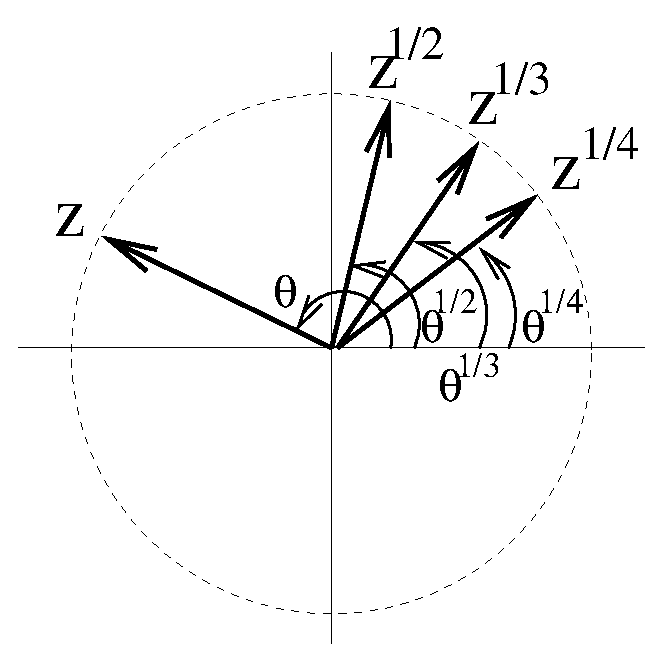
\includegraphics[width=7cm,height=7cm]{images/root.eps}
\caption[Roots of Complex numbers]{The $n$th root of a
complex number is an angle which 1/$n$th the original number.}
\end{center}
\end{figure}
At times it is useful to have the formula for a root of a complex 
number in rectangular form. While this can't be done in general, 
the square root is tractable:
\begin{equation}
\sqrt{a+ib} = 
\sqrt{\frac{\sqrt{a^2 + b^2} +a}{2}} +isgn(b)
\sqrt{\frac{\sqrt{a^2 + b^2} -a}{2}}
\end{equation}
where $sgn(b)$ is the signum function, which is also known
as the sign of $b$.  The signum function is generally 
defined as $b/|b|$.  We define $sgn(0)$ to be unity.

\section{The Problem that ``Can't Be Done''}
In pre-calculus and even in calculus, you may have been told
that calculating the $arccos$ of a number greater than 1
can't be done.  Since the $cos$ function oscillates between
-1 and 1, calculating $arccos(3)$ would be ``difficult.''
When I ask my calculator to calculate $arccos(3)$, it says
``Error 0.''

Of course the calculator and the early math courses are
restricting themselves to the real number system.\footnote{Your 
calculator may not have this restriction.}
The $arccos(3)$, for example, is just a complex number.
In fact, it is pure imaginary, as we will now show.


\begin{example}
\textbf{Inverse Trig Functions}\\
Calculate $arccos(3)$.
\end{example}

\begin{proof}
let 
\begin{equation}
y uiv arccos(3)
\end{equation}, then $cos(y) = 3$.
But from the Euler Relation, the $cos$ function
can be written as a sum of complex exponentials:
\begin{equation}A
\frac {e^{iy} + e^{-iy}}{2} = 3
\end{equation}
A
Multiplying both sides by $2e^{iy}$, and moving
all terms to the left hand side of the equation
results in
\begin{equation}A
{\left ( e^{iy} \right ) }^2 - 6e^{iy} +1=0
\end{equation}A
which is a quadratic equation in $e^{iy}$.  The
solutions are
\begin{equation}A
e^{iy}=3 \pm 2 \sqrt{2}
\end{equation}A
Taking the natural log of both sides and multiplying by
$-i$ results in
\begin{equation}A
y = -i ln(3 \pm 2 \sqrt{2})
\end{equation}A
\end{proof}

%%%%%%%%%%%%%%%%%%%%%%%%%%%%%%%%%%%%%%%%%%%%%%%%%%%%%%%%
%%%%%%%%%%%%%%%%%%%%%%%%%%%%%%%%%%%%%%%%%%%%%%%%%%%%%%%%

\section{PROBLEMS}

\begin{problems}
Separate the following into real and imaginary parts:\\
a)      $\frac{3+i4}{5+i7}$\\
b)      $(3+i4) +i(4+i5) + (2+i3)(4+i5)^2$\\
c)      $tan(3+i4)$\\
d)      $e^{3+i4}$\\
e)      $\sqrt{1+i2}$\\
f)      $ln(3+i4)$\\
g)      $sin^{-1} (3)$\\
h)      $i^i$\\
        Hint: $i$ can be thought of as a complex number in rectangular form.\\
i)      There are an infinite number of values for $i^i$, what are they?\\
        Hint: $e^{i \theta} = e^{i( \theta + 2n \pi )}$\\
\end{problems}

\begin{problems}
Consider a series AC electrical circuit with two resistors
and a capacitor.
\begin{figure}[h]
\begin{center}
\includegraphics[width=7cm,height=3cm]{images/RRC1.eps}
\caption[RC Circuit]{A simple AC circuit.}
\end{center}
\end{figure}
The output complex voltage is related to the input complex voltage by 
the voltage divider law
\[
{\hat{V}}_{out} = \frac{R_2}{R_1 + R_2 -i/(\omega C)} {\hat{V}}_{in}
\]
If $R_1 = 100 \Omega $, $R_2= 200 \Omega $, $C = 50 {\mu}F$, and 
$\omega = 2 \pi (60)$ cycles/s, and ${\hat{V}}_{in} = 100 V$, 
then what is the \\

a)      magnitude of the output voltage,\\
b)      phase of the output voltage.\\
c)      plot $| {\hat{V}}_{out} / {\hat{V}}_{in} |$ as a function 
of differents $\omega$'s.
\end{problems}

\begin{problems}
If $\Psi$ is the wave function from the Schr\"{o}dinger equation, then
the probability density of finding a particle at a particular
place is given by $P(x) = \Psi ^* \Psi$.  Suppose that you
have solved the Schr\"{o}dinger equation for a given potential
functions, and you find that
\[
\Psi (x) = \frac{p}{1+qx^2}
\]
where $p=p_r +i p_i$, $q=q_r + iq_i$ are complex constants, and
$P=p^*p$, and $Q=q^*q$.
Compute the probability density distribution in this case.
(Note: $x$ is a real variable).
\end{problems}


\begin{problems}
One problem of interest is the writing of
the $n^{th}$ power of $cos$ into a Fourier series.
Using trigonometric identities it is generally difficult to
prove that
\[
cos^m(\omega t) = \frac{1}{2^m}
\sum_{k=0}^m \frac{m!}{k!(m-k)!} cos[(m-2k) \omega t]
\]
Use the Euler relation to derive the above result\footnote {As the
student may be aware, the
binomial theorem is $(a+b)^m = \sum_{k=0}^m \frac{m!}{k!(m-k)!} 
a^k b^{m-k}$}.
\end{problems}

\begin{problems}
Plot the following phasors tail-to-tip on a piece of graph
paper:\\
\begin{eqnarray*}
2 - \sqrt{29}e^{-i tan^{-1}(5/2)} + (\sqrt{34}/5)e^{+i tan^{-1}(3/5)} -2 + 
(\sqrt{136}/5)e^{-i tan^{-1}(3/5)}
\end{eqnarray*}
\begin{eqnarray*}
- \sqrt{5}e^{-i tan^{-1}(2)} 
- \sqrt{5}e^{+i tan^{-1}(2)} 
+ (\sqrt{34}/5)e^{+i tan^{-1}(3/5)} -
(\sqrt{29}/5)e^{+i tan^{-1}(5/2)} +2
\end{eqnarray*}
Hints: 1)  Start near the bottom middle of your graph paper.
2)  The sum of the complex numbers is zero, so the last
phasor should end at the same place your first complex number
started.
\end{problems}
\begin{problems}
The complex propagation constant for an electromagnetic
wave propagating in a conductive medium can be obtained
from the formula
\begin{eqnarray*}
        {k_0}^2 & = &  {\omega}^2 \mu \epsilon - i \mu \sigma \omega \\
        & \equiv & (\beta_0 - i\alpha_0 )^2 
\end{eqnarray*}
where ${\beta}_0$ is the propagation constant and ${\alpha}_0$
is the loss per length.  
\begin{description}
        \item[a)] If the skin depth
                $\delta = 1/ {\alpha}_0$, then
                obtain an analytical expression for $\delta$ in terms of
                $\omega$, $\mu$, $\epsilon$, and $\sigma$.
        \item[b)] Simply you expression for 
                $\frac{\sigma}{\omega \epsilon} << 1$.
\end{description}
\end{problems}

\begin{problems}
Use the Euler Relation to derive the trigonometric identity for
the $sin$ of the sum of two different angles:  $sin(a+b)$.
\end{problems}

\begin{problems}
Often times books show a proof of Euler's Identity by
looking at the Taylor series expansion for $sin(x)$ and
$cos(x)$, comparing it to the expansion for $e^x$ and
saying ``Tada, it works!''  Here the goal is to 
$derive$ the Euler relation,
assuming that we know a little bit about differential
equations.  Put another way, we don't want to just show
that it happens to work, but that it $must$ work.
First, we consider the following differential
equation which represents simple harmonic motion such
as from a pendulum (small angles) or a spring:
\[
\frac{d^2y}{dt^2} + {\omega}^2 y(t) = 0
\]
Complete the following steps of the derivation:\\
\begin{description}
\item[a)]Show that $y(t)= a sin( \omega t) + b cos( \omega t)$
are solutions to the differential equation.
\item[b)]Apply the boundary conditions $y(0)=y_0$ and
$y^{\prime}(0) = y^{\prime}_0$ to this solution.
\item[c)]Show that $y(t)= A e^{i \omega t} + B e^{-i \omega t}$
are solutions to the differential equation.
\item[d)]Apply the boundary conditions $y(0)=y_0$ and
$y^{\prime}(0) = y^{\prime}_0$ to this solution.
\item[e)]Since the differential equation is second order, it
has only two independent solutions.  Thus coefficients of
the $y_0$ terms in the two equations must be equal to each
other.  Set them equal to each other, and solve for
$e^{i \omega t}$.
\end{description}
\end{problems}

\begin{problems}
Make separate plots of the following roots 
as phasors in the complex plane:\\
a)      $z^2 = 1$\\     
b)      $z^3 = 1$\\     
c)      $z^4 = 1$\\     
d)      $z^5 = 1$\\     
e)      $z^3 = \frac{1+i}{\sqrt{2}}$\\
\end{problems}
